
\chapter{Regular Expressions}

A regular expression is a compact notation for representing a collection of strings.
What makes regular expressions so powerful is that a \keyword{single} regular expression can represent an \keyword{unlimited} number of strings.


Regexes (REGular EXpression) are used for five main purposes:
\begin{description}
\item[Parsing] 
\item[Searching] 
\item[Searching and replacing] 
\item[Spliting strings] 
\item[Validation] 
\end{description}

\begin{tcolorbox}
  The core of regular expression is \keyword{matchding}.
  All the above five purposes is based on the matching.
\end{tcolorbox}


\section{Python's regular expression language}

\begin{tcolorbox}
  \textbf{bold font} for regular expression;
  \underline{underlining} for matching;
  \mikebl{shading} for capture;
\end{tcolorbox}

\subsection{Character and character classes}

The simplest expressions are just literal characters, such as \keyword{a} or \keyword{5}, and if no quantifier is explicitly given it is taken to be ``match one occurrence''.

For example, the regex \textbf{mike} consists of four expressions, each implicitly quantified to match once, so it matches one \textit{m} followed by one \textit{i} followed by one \textit{k} followed by one \textit{e}, and hence matches the string \underline{mike} and \underline{mike}chyson.


Although most characters can used as literals, some are ``special characters'' -- these are symbols in the regex language and so must be escaped by preceding them with a backslash(\textbackslash{}) to use as literals.
The speical characters are \verb-\.^$?+*{}[]()|-.
Most of Python's standard string escapes can also be sued within regexes, for example \verb|\n| for newline and \verb|\t| for tab, as well as hexadecimal escapes for characters using the \verb|\xHH|, \verb|\uHHHH| and \verb|\UHHHHHHHH| syntaxes.



In many cases, rather than matching one particular character we want to match any one of a set of characters.
This can be achieved by using a \keyword{character class} -- one or more characters enclosed in square brackets.
(This has nothing to do with a Python class, and is simply the regex term for ``set of characters''.)
A character class is an expression, and like any other expression, if not explicitly quantified it matches exactly one character (which can be any of the characters in the character class).

For example, the regex \textbf{r[ea]d} matches both \underline{red} and \underline{rad}, but not read.


For convenience we can specify a range of character using a hyphen, so the regex \textbf{[0-9]} matches a digit.
It is possible to negate the meaning of a character class by following the opening bracket with a caret, so \textbf{[\^{}0-9]} matches any character that is not a digit.



\begin{tcolorbox}
  Note that inside a character class, apart from \textbackslash, the special characters lose there special meaning, although in the case of \^{} it acquires a new meaning (negation) if it is the first character in the character class, and otherwise is simply a literal caret.
  Alse, \--{} signifies a character range unless it is the first character, in which case it is a literal hyphen.
\end{tcolorbox}


Since some sets of characters are required so frequently, several have shorthand forms, as shown in table \ref{tab:character-class-shorthands}.
With one exception that the shorthands can be used inside character sets, so example, the regex \textbf{[\textbackslash dA-Fa-f]} matches any hexadecimal digit.
The exception is . which is a shorthand outside a character class but matches a literal . inside a character class.

\begin{table}[!ht]
  \centering
  \begin{tabular}{lp{0.7\columnwidth}}
    \toprule
    \head{Symbol} & \head{Meaning} \\
    . & Matches any character except newline; or any character at all with the \verb|re.DOTALL| flag; or inside a character class matches a literal . \\
    \textbackslash d & Matches a Unicode digit; or \textbf{[0-9]} with the \verb|re.ASCII| flag \\
    \textbackslash D & Matches a Unicode nondigit; or \textbf{[\^{}0-9]} with the \verb|re.ASCII| flag \\
    \textbackslash s & Matches a Unicode whitespace; or \textbf{[ \textbackslash t\textbackslash n\textbackslash r\textbackslash f\textbackslash v]} with the \verb|re.ASCII| flag \\
    \textbackslash S & Matches a Unicode nonwhitespace; or \textbf{[\^{} \textbackslash t\textbackslash n\textbackslash r\textbackslash f\textbackslash v]} with the \verb|re.ASCII| flag \\
    \textbackslash w & Matches a Unicode ``word'' character; or \textbf{[a-zA-Z0-9\_]} with the \verb|re.ASCII| flag \\
    \textbackslash W & Matches a Unicode non-``word'' character; or \textbf{[\^{}a-zA-Z0-9\_]} with the \verb|re.ASCII| flag \\
    \bottomrule
  \end{tabular}
  \caption{Character class shorthands}
  \label{tab:character-class-shorthands}
\end{table}



\subsection{Quantifiers}

A quantifier has the form {m,n} where m and n are the minimum and maximum times the expression the quantifier applies to must match.
For example, both \textbf{e{1,1}e{1,1}} and \textbf{e{2,2}} match f\underline{ee}l, but neither matches felt.



Writing a quantifier after every expression would soon become tedious.
Fortunately, the regex language supports several convenient shorthands.
If only one number is given in the quantifier it is taken to be both the minimum and the maximum, so \textbf{e{2}} is the same as \textbf{e{2,2}}.
If no quantifier is explicitly given, it is assumed to be one.



\begin{table}[!ht]
  \centering
  \begin{tabular}{lp{0.7\columnwidth}}
    \toprule
    \head{Syntax} & \head{Meaning} \\
    \midrule
    e? or e\{0,1\} & Greedily match zero or one occurence of expression e \\
    e+ or e\{1,\} & Greedily match one or more occurences of expression e \\
    e* or e\{0,\} & Greedily match zero or more occurences of expression e \\
    e\{m\} & Match exactly m occurences of expression e \\
    e\{m,\} & Greedily match at least m occurences of expression e \\
    e\{,n\} & Greedily match at most n occurences of expression e \\
    e\{m,n\} & Greedily match at least m and at most n occurences of expression e \\
    \bottomrule
  \end{tabular}
  \caption{Regular Expression Quantifiers}
  \label{tab:regular-expression-quantifiers}
\end{table}



By default, all quantifiers are \textit{greedy} -- they match as many characters as then can.
We can make any quantifiers nongreedy (also called \textit{minimal}) by following it with a ? symbol.
The question mark has two different meanings -- on its own it is a shorthand for the \textbf{\{0,1\}} quantifier, and when it follows a quantifier it tells the quantifier to be nongreedy.)



\subsection{Grouping and capturing}

In practical applications we often need regexes that can match any one of two or more alternatives, and we often need to capture the match or some part of the match for further processing.
Also, we sometimes want a quantifier to apply to several expressions.
All of these can be achieved by grouping with (), and in the case of alternatives using alternation with |.
For example,
the regex \textbf{air(craft|plane)|jet} will match any text that containing ``aircraft'' or ``airplace'' or ``jet''.


Parentheses serve two different purpose -- to group expressions and to capture the text that matches an expression.
We use the term \textit{group} to refer to a grouped expression whether it captures or not, and \textit{capture} and \textit{caputure group} to refer to a captured group.
For example,
The regex \textbf{(aircraft|airplane|jet)} would not only match any of the three expressions, but would also capture whichever one was matched for later reference.

We can switch off the capturing effect by following on opening parenthesis with \textbf{`?:}.
For example,
\textbf{(?:aircraft|airplane|jet)}.



A grouped expression is an expression and so can be quantified.
Like any other expression the quantity is assumed to be one unless explicitly given.

For example,
the regex \textbf{(\textbackslash w+)=(.+)} will match \underline{\mikebl{topic}=\mikebl{ physical geography}} with the two captures shown shaded.
The regex \textbf{[ \textbackslash t]*(\textbackslash +)[ \textbackslash t]*=[ \textbackslash t]*(.+)} will match \underline{\mikebl{topic} = \mikebl{physical geography}}.
The later regex keep the whitespace matching parts outside the capturing parentheses, and to allow for lines that have no whitespace at all.



Captures can be referred to using \textit{backreferences}, that is, by referring back to an earlier capture group\footnote{Backreferences cannot be used inside character classes, that is, inside [].}.
One syntax for backreferences inside regexes themselves is \textit{\textbackslash i} where \textit{i} is the capture number.
Captures are numbered starting from one and increasing by one going from left to right as each new (capturing) left parenthesis is encountered. 
For example, to simplistically match duplicated words we can use the regex \textbf{(\textbackslash w+)\textbackslash s+\textbackslash 1} which matches a ``word'', then at least one whitespace, and then the same word as was captured.
(Capture number 0 is created automatically without the need for parentheses; it holds the entire match.)



In long or complicated regexes it is often more convenient to use names rather than numbers for captures.
This can also make maintenance easier since adding or removing capturing parentheses may change the numbers but won’t affect names.
To name a capture we follow the opening parenthesis with \textbf{?P<}\textit{name}\textbf{>}.
For example, \textbf{(?P<key>\textbackslash w+)=(?P<value>.+)} has two captures called ``key'' and ``value''.
The syntax for backreferences to named captures inside a regex is \textbf{(?=}\textit{name}\textbf{)}.
For example, \textbf{(?P<word>\textbackslash w+)\textbackslash s+(?P=word)} matches duplicate words using a capture called ``word''.


\subsection{Assertions and flags}

One problem that affects many of the regexes is that they can match more or different text than we intended.
For example, the regex \textbf{aircraft|airplane|jet} will match ``waterjet'' and ``jetski'' as well as ``jet''.
This kind of problem can be solved by using assertions.
An assertion does not match any text, but instead says something about the text at the point where the assertion occurs.



Some assertions are shown in Table \ref{tab:assertions}
\begin{table}[!ht]
  \centering
  \begin{tabular}{lp{0.7\columnwidth}}
    \toprule
    \head{Symbol} & \head{Meaning} \\
    \midrule
    \^{} & Matches at the start; also matches after each newline with the \verb|re.MULTILINE| flag \\
    \$ & Matches at the end; also matches before each newline with the \verb|re.MULTILINE| flag \\
    \textbackslash A & Matches at the start \\
    \textbackslash b & Matches at a ``word'' boundary \\
    \textbackslash B & Matches at a non-``word'' boundary \\
    \textbackslash Z & Matches at the end \\
    (?=e) & Matches if the expression e matches at this assertion but does not advance over it -- called lookahead or positive lookahead \\
    (?!e) & Matches if the expression e does not match at this assertion and does not advance over it -- called negative lookahead \\
    (?<=e) & Matches if the expression e matches immediately before this assertion -- called positive lookbehind \\
    (?<!e) & Matches if the expression e does not match immediately before this assertion -- called negative lookbehind
  \end{tabular}
  \caption{Regular Expression Assertions}
  \label{tab:assertions}
\end{table}


The key value regex is as follows:
\begin{lstlisting}
  r'''^[ \t]*(?P<key>\w+)[ \t]*=[ \t]*(?P<value>[^\n]+)(?<![ \t])'''
\end{lstlisting}



It looks quite complicated.
One way to make it more maintainable is to include comments in it.
This can be done by adding inline comments using the syntax (\verb|?#the comment|), but in practice comments like this can easily make the regex even more difficult to read.
A much nicer solution is to use the \verb|re.VERBOSE| flag —- this allows us to freely use whitespace and normal Python comments in regexes, with the one constraint that if we need to match whitespace we must either use \textbf{\textbackslash s} or a character class such as \textbf{[ ]}.
Here’s the \textit{key=value} regex with comments:
\begin{lstlisting}
r'''
^[ \t]*              # start of lien and optional leading whitespace
(?P<key>\w+)         # the key text
[ \t]*=[ \t]*        # the equals with optional surrounding whitespace
(?P<value>[^\n]+)    # the value text
(?<![ \t])           # negative lookbehind to avoid trailing whitespace
'''
\end{lstlisting}




Suppose we want to extract the filenames referred to by the \verb|src| attribute in HTML \verb|img| tags.
\begin{lstlisting}
r'''
<img\s+                              # start of the tag
[^>]*?                               # any attributes that precede the src
src=                                 # start of the src attribute
(?:
     (?P<quote>["'])                 # opening quote
     (?P<qimage>[^\1>]+?)            # image filename
     (?P=quote)                      # closing quote matching the opening quote
|
     (?P<uimage>[^"' >]+             # unquoted image filename
)
[^>]*?                               # any attribute that follow the src
>     
'''
\end{lstlisting}

Note that to refer to the matching quote inside the character class we have to use a numbered backreference \textbf{\textbackslash 1}, instead of \textbf{(?=quote)}, since only numbered backreference work inside character classes.


\section{The regular expression module}

The \verb|re| module provides two ways of working with regexes:
\begin{enumerate}
\item Use the functions listed in Figure \ref{fig:regex-first-way}
\item Compile the regex and call compiled regex methods in Figure \ref{fig:regex-second-way}
\end{enumerate}

\begin{figure}[!ht]
  \centering
  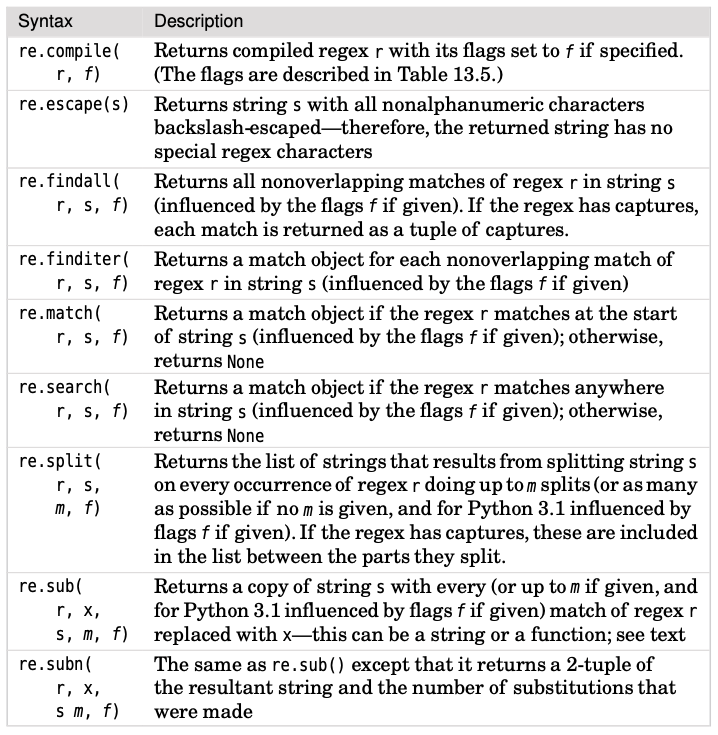
\includegraphics[width=\textwidth]{pics/regex-first-way}
  \caption{The Regular Expression Module’s Functions}
  \label{fig:regex-first-way}
\end{figure}


\begin{figure}[!ht]
  \centering
  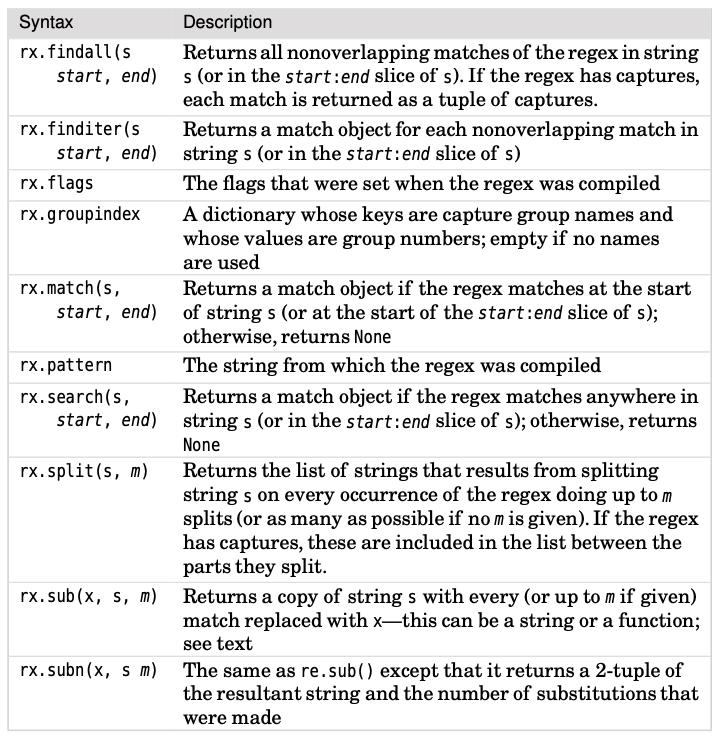
\includegraphics[width=\textwidth]{pics/regex-second-way}
  \caption{Regular Expression Object Methods}
  \label{fig:regex-second-way}
\end{figure}


\begin{figure}[!ht]
  \centering
  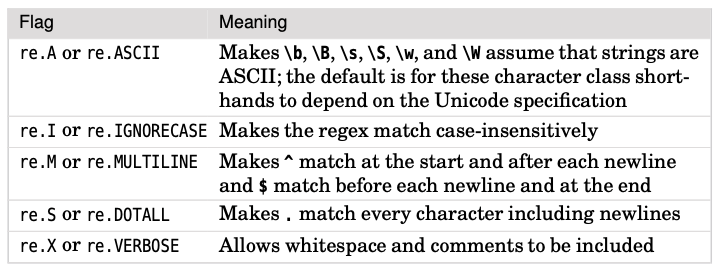
\includegraphics[width=\textwidth]{pics/regex-flag}
  \caption{The Regular Expression Module's Flags}
\end{figure}


For example (search):
\begin{lstlisting}
import re

# manner 1
text = '#C0C0AB'
match = re.search(r'#[\dA-Fa-f]{6}\b', text)

# manner 2
color_re = re.compile(r'#[\dA-Fa-f]{6}\b')
match = color_re.search(text)

# flag
match = re.search(r'#[\dA-F]{6}\b', text, re.IGNORECASE)
match = re.search(r'(?i)#[\dA-F]{6}\b', text)
\end{lstlisting}


The methods provided by match objects are listed in Figure \ref{fig:match-object-methods}
\begin{figure}[!ht]
  \centering
  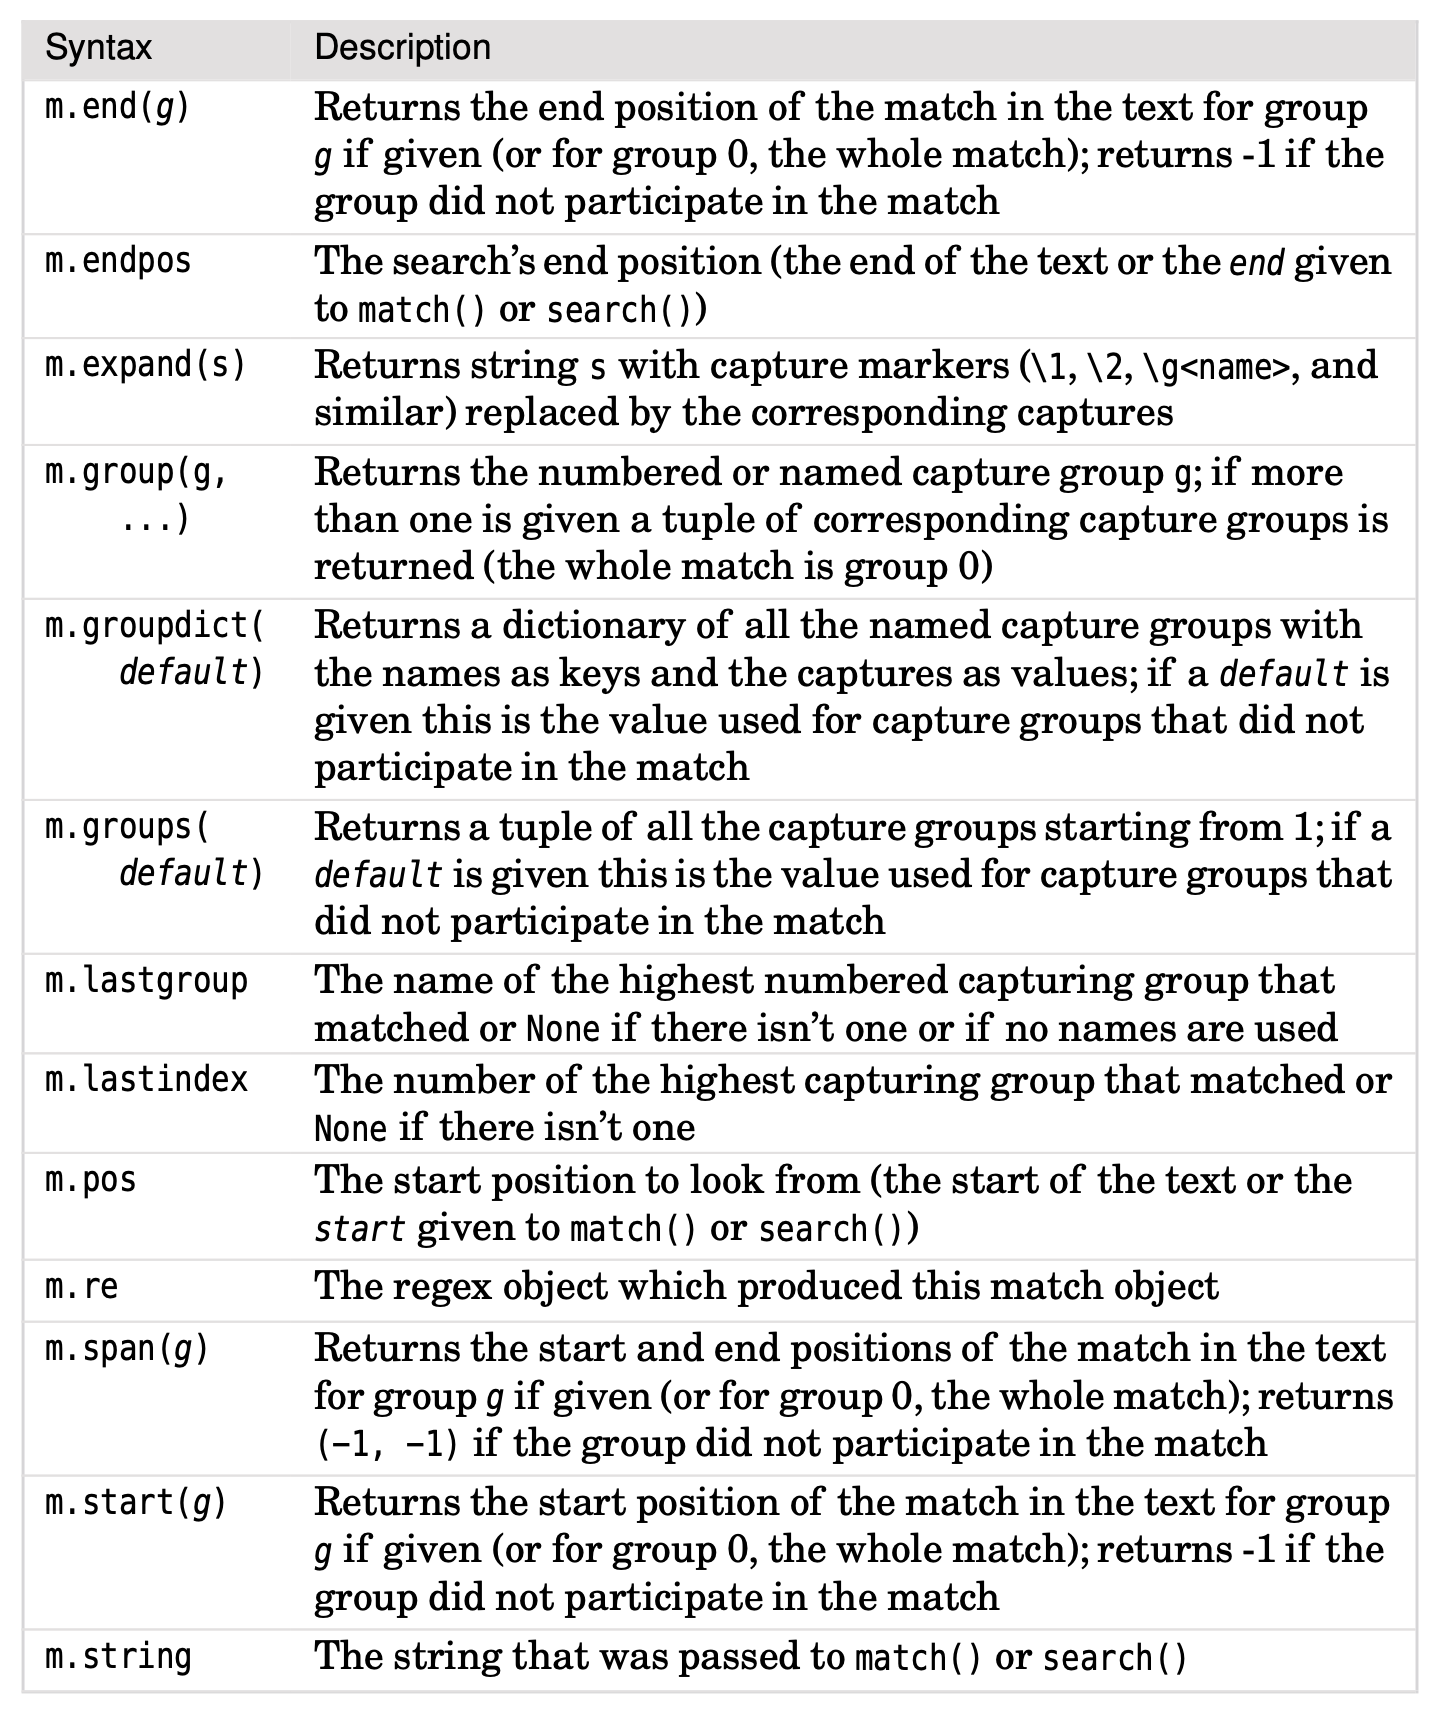
\includegraphics[width=\textwidth]{pics/match-object-methods}
  \caption{Match Object Attribute and Methods}
  \label{fig:match-object-methods}
\end{figure}

Example (check duplicate words):
\begin{lstlisting}
text = "one and and two let's say"
double_word_re = re.compile(r"\b(?P<word>\w+)\s+(?P=word)(?!\w)", re.IGNORECASE)
double_word_re = re.compile(r"\b(?P<word>\w+)\s+(?P=word)\b", re.IGNORECASE) # same to the above
for match in double_word_re.finditer(text):
    print(f'{match.group("word")} is duplicated')
# and is duplicated
\end{lstlisting}


Example (extract image filenames):
\begin{lstlisting}
text = '''
<img src="/images/stickman.gif" alt="Stickman" width="24" height="39">
<img src="https://www.w3schools.com/images/lamp.jpg" alt="Lamp" width="32" height="32">
'''
image_re_text = r'''
<img\s+                              # start of the tag
[^>]*?                               # any attributes that precede the src
src=                                 # start of the src attribute
(?:
     (?P<quote>["'])                 # opening quote
     (?P<qimage>[^\1>]+?)            # image filename
     (?P=quote)                      # closing quote matching the opening quote
|
     (?P<uimage>[^"' >]+)            # unquoted image filename
)
[^>]*?                               # any attribute that follow the src
>     
'''
image_re = re.compile(image_re_text, re.IGNORECASE | re.VERBOSE)
image_files = []
for match in image_re.finditer(text):
    image_files.append(match.group("qimage") or match.group("uimage"))
for image_file in image_files:
    print(image_file)
# /images/stickman.gif
# https://www.w3schools.com/images/lamp.jpg  
\end{lstlisting}



Example (convert html to text):
\begin{lstlisting}
def html2text(html_text):
    def char_from_entity(match):
        code = html.entities.name2codepoint.get(match.group(1), 0xFFFD)
        return chr(code)

    # (?s) math . include newline
    text = re.sub(r"(?s)<!--.*?-->", "", html_text)  # HTML comments
    text = re.sub(r"<[Pp][^>]*?>", '\n\n', text)  # opening paragraph tags
    text = re.sub(r"<[^>]*?>", '', text)  # any tag
    text = re.sub(r"&#(\d+);", lambda m: chr(int(m.group(1))), text)  # &#165; for ¥
    text = re.sub(r"&([A-Za-z]+);", char_from_entity, text)  # named entities
    text = re.sub(r"\n(?:[ \xA0\t]+\n)+", '\n', text)  # linesthat contain only whitespace
    # Replace sequences of two or more newlines with exactly two newlines
    text = re.sub(r"\n\n+", '\n\n', text.strip())
    return text  
\end{lstlisting}


Example (switch name order in fullname):
\begin{lstlisting}
import re

# from Forename Middlename1 ... MiddlenameN Surname
# to Surname,ForenameMiddlename1...MiddlenameN
names = ['Mike Ming Chyson', 'Maël Ming Li']
new_names = []
for name in names:
    # name = re.sub(r"(\w+(?:\s+\w+)*)\s+(\w+)", r"\2, \1", name)
    name = re.sub(r"(?P<forenames>\w+(?:\s+\w+)*)"
                  r"\s+(?P<surname>\w+)",
                  r"\g<surname>, \g<forenames>",
                  name)
    new_names.append(name)
for name in new_names:
    print(name)
# Chyson, Mike Ming
# Li, Maël Ming  
\end{lstlisting}


Example (detect encoding):
\begin{lstlisting}
import re

binary = b''

re_binary = r"""
# A lookbehind assertion that says that the
# match cannot be preceded by a hyphen or a word character.
(?<![-\w]) 
(?:(?:en)?coding|charset)  # encoding|coding|charset
(?:=(["'])?([-\w]+)(?(1)\1)
|:\s*([-\w]+))
""".encode('utf8')
match = re.search(re_binary, binary, re.IGNORECASE | re.VERBOSE)
encoding = match.group(match.lastindex) if match else b'utf8'
\end{lstlisting}

Example (split text based on whitespace):
\begin{lstlisting}
text = 'hello world'
re.split(r"\s+", text)
# same to
text.split()  
\end{lstlisting}